\section{Ingeniería de detalle}\label{sec:ingdetalle}

% Es el conjunto de documentación técnica completa del proyecto que
% permite que la ejecución de éste sea entregada a un tercero y éste
% pueda efectuar la Instalación y Puesta en Marcha con mínimas
% variaciones.

% La Instalación y Puesta en marcha de un proyecto no necesariamente
% debe ser ejecutada por el grupo de trabajo que prepara la Ingeniería
% de Detalle. El ejecutor puede ser otra sección dentro de la misma
% Empresa o una Empresa contratista (Outsourcing). Por este motivo la
% Ingeniería de detalle debe ser completa y muy precisa. No deben quedar
% detalles sin definir.

% Dentro de la Ingeniería de detalle de un proyecto, y dependiendo de la
% naturaleza de éste, se pueden incluir los siguientes elementos:

% Planos de planta de las estaciones, especificando ubicación y
% dimensiones de los racks que alojarán a los equipos nuevos Layout de
% los equipos, esto es, planos frontales de los racks indicando la
% disposición de los equipos.

% Diagramas en bloque de los equipos indicando las interconexiones de
% los diferentes módulos (no se trata de los diagramas de circuitos
% electrónicos de cada tarjeta, información que los fabricantes no
% suelen entregar, sino que de las conexiones externas entre las
% diferentes tarjetas, para conseguir que los equipos trabajen en la
% forma deseada).

% Diagrama de cross-conexiones entre las diferentes interfaces de línea
% y las puertas tributarias de los equipos.  Plan de sincronización de
% la Red Planos de Planta Externa Memorias de cálculo
 
 
% El último elemento requiere de explicaciones adicionales.
 
% Una Memoria de Cálculo, como su nombre indica, es el resultado de los
% análisis y cálculos que efectúa un ingeniero especialista en una
% materia para determinar la forma correcta como debe ejecutarse una
% parte del proyecto para que el sistema funcione correctamente y de
% acuerdo a lo esperado.
 
% La memoria de cálculo puede ser de varios tipos según el
% proyecto. Algunos ejemplos:
 
% Memoria de cálculo de malla de tierra. Arroja como resultado
% especificaciones sobre la geometría de la malla, profundidad y número
% de las barras de cobre que deben enterrarse, valor de resistividad del
% terreno al cual debe llegarse.
 
% Memoria de cálculo de un radio enlace. Incluye un perfil del enlace,
% cálculos de niveles de señal, atenuaciones de las guías de onda y
% filtros, ganancia de las antenas, potencias de salida de los
% transmisores y nivel de recepción. Pero lo más importante es el
% cálculo de predicción de comportamiento del enlace en el peor mes del
% año, esto es \% del tiempo que el enlace estará indisponible (Tasa de
% error peor que 1E-03) y \% del tiempo que el enlace estará degradado
% (Tasa de error peor que 1E-06). Todos los métodos de cálculo y valores
% límites para los porcentajes mencionados están detallados por el ITU.
 
% Memoria de cálculo de enlaces por fibra óptica. Este tema es de
% importancia para el proyecto que les corresponde desarrollar. estos
% cálculos incluyen: balance de potencia; cálculo de razón señal a ruido
% óptica (OSNR) y cálculos de dispersión.
 
% Los resultados de estos cálculos determinan el diseño de la red y por
% lo tanto tiene impacto en el CAPEX y OPEX del proyecto: tipo de
% interfaces ópticas (estándar, de alta potencia, Ultra alta potencia),
% necesidad de usar Amplificadores Ópticos de Línea (OLA) o
% Regeneradores intermedios en un enlace.
 
% El impacto en el CAPEX es claro, si el diseño arroja que es necesario
% incluir una estación regeneradora en medio de un enlace entre
% estaciones ya existentes, el costo del proyecto se eleva notablemente.
 
% Por otra parte, un diseño muy audaz puede significar una reducción del
% margen disponible en el enlace, lo cual ante una degradación menor del
% cable de fibra puede hacer que el enlace se corte o degrade, obligando
% a efectuar mantenimiento con más frecuencia y elevando el OPEX.
 
% Memoria de cálculo de una torre. En un proyecto que incluya enlaces de
% microondas y emplazamiento de radio estaciones nuevas con sus
% receptivas torres, se debe incluir el cálculo de la estructura de la
% torre para asegurar su resistencia al peso de las antenas, al viento,
% etc. Naturalmente este cálculo cae dentro de las responsabilidades de
% un Ingeniero Civil no Eléctrico.

En esta sección se presentará la ingeniería de detalle para el
proyecto de implementación de red óptica utilizando \emph{DWDM} y
\emph{ROADM} con \emph{WSS} basado en un enfoque probabilístico para
diseño de caminos óptimos a partir de valores esperados del
\emph{SLA}.

La ingeniería de detalle expuesta aquí es una recopilación de todos
los documentos técnicos que se requieren para la instalación física de
los equipos y la programación de los \emph{ROADM}. Esta recopilación
se basa en el diseño final seleccionado de entre las propuestas de los
proveedores en la sección \ref{sec:ppfinal}.

\subsection{Diagramas de conexión ROADM}
\label{sec:diagramasroadm}

El detalle de las conexiones de equipos en cada uno de los \emph{DC}
se presenta en las siguientes secciones.

\subsubsection{Conexión ROADM ``Ciudad de los valles''}
\label{sec:drcdv}

\begin{figure}[H]
  \centering
  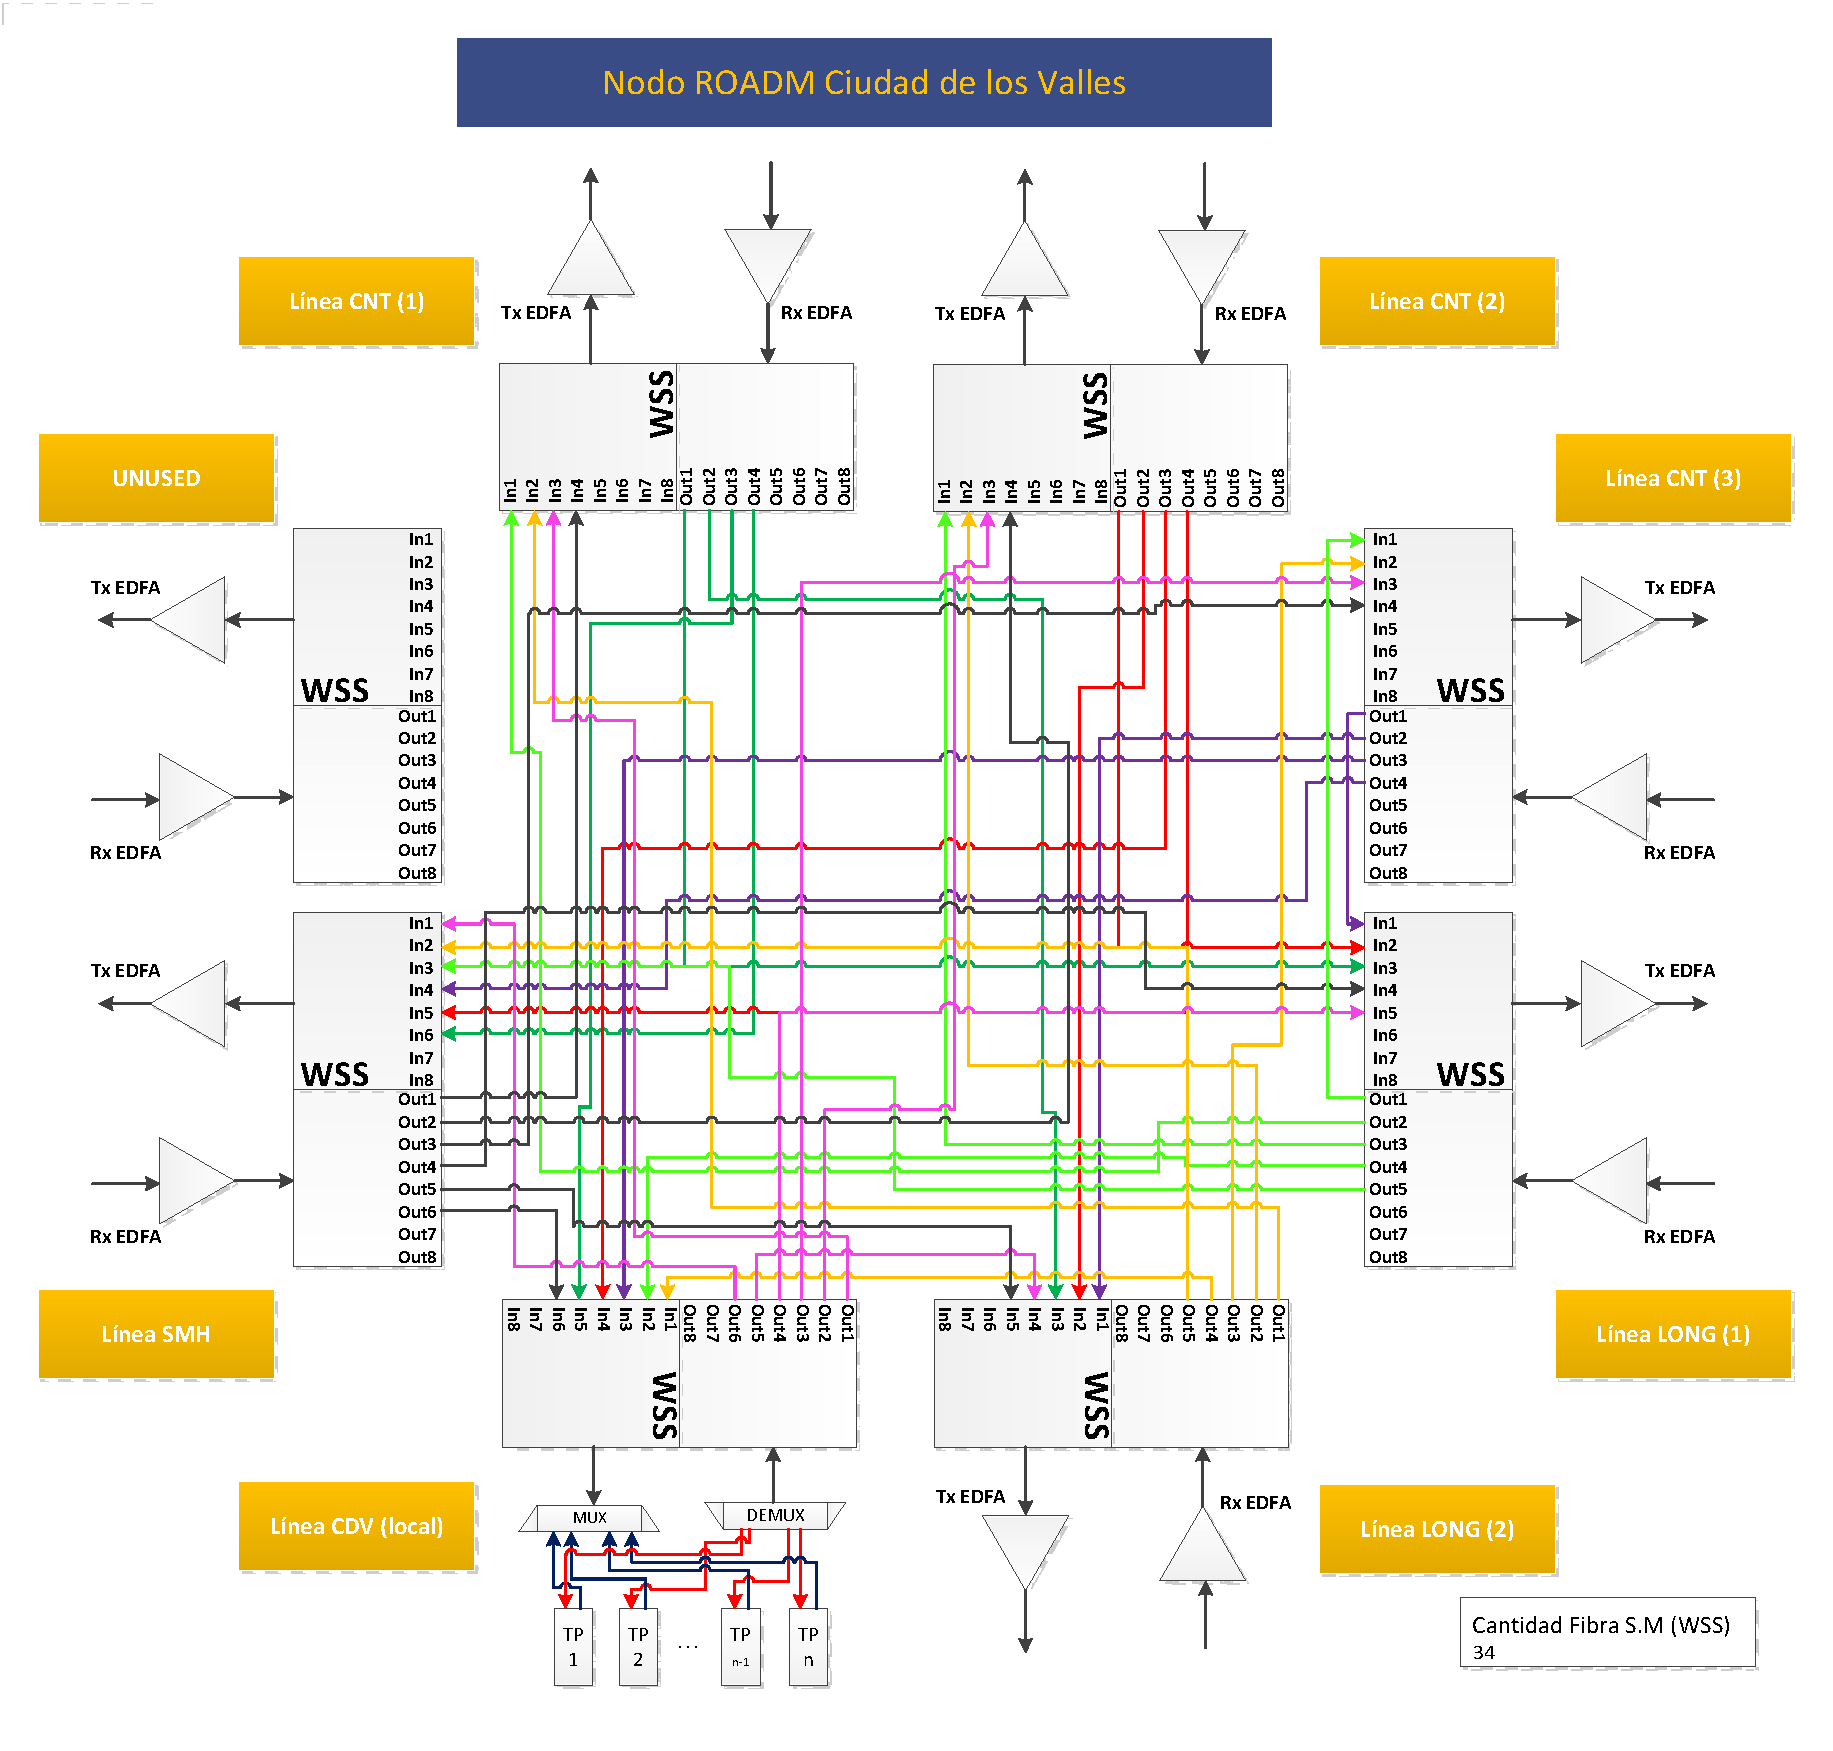
\includegraphics[width=17cm]{Imagenes/CDV.pdf}
  \caption{Diagrama de conexión de equipos para infrastructura ROADM en ``Ciudad de los valles''}
  \label{fig:drcdv}
\end{figure}

\subsubsection{Conexión ROADM ``Central nacional de telecomunicaciones''}
\label{sec:drcnt}

\begin{figure}[H]
  \centering
  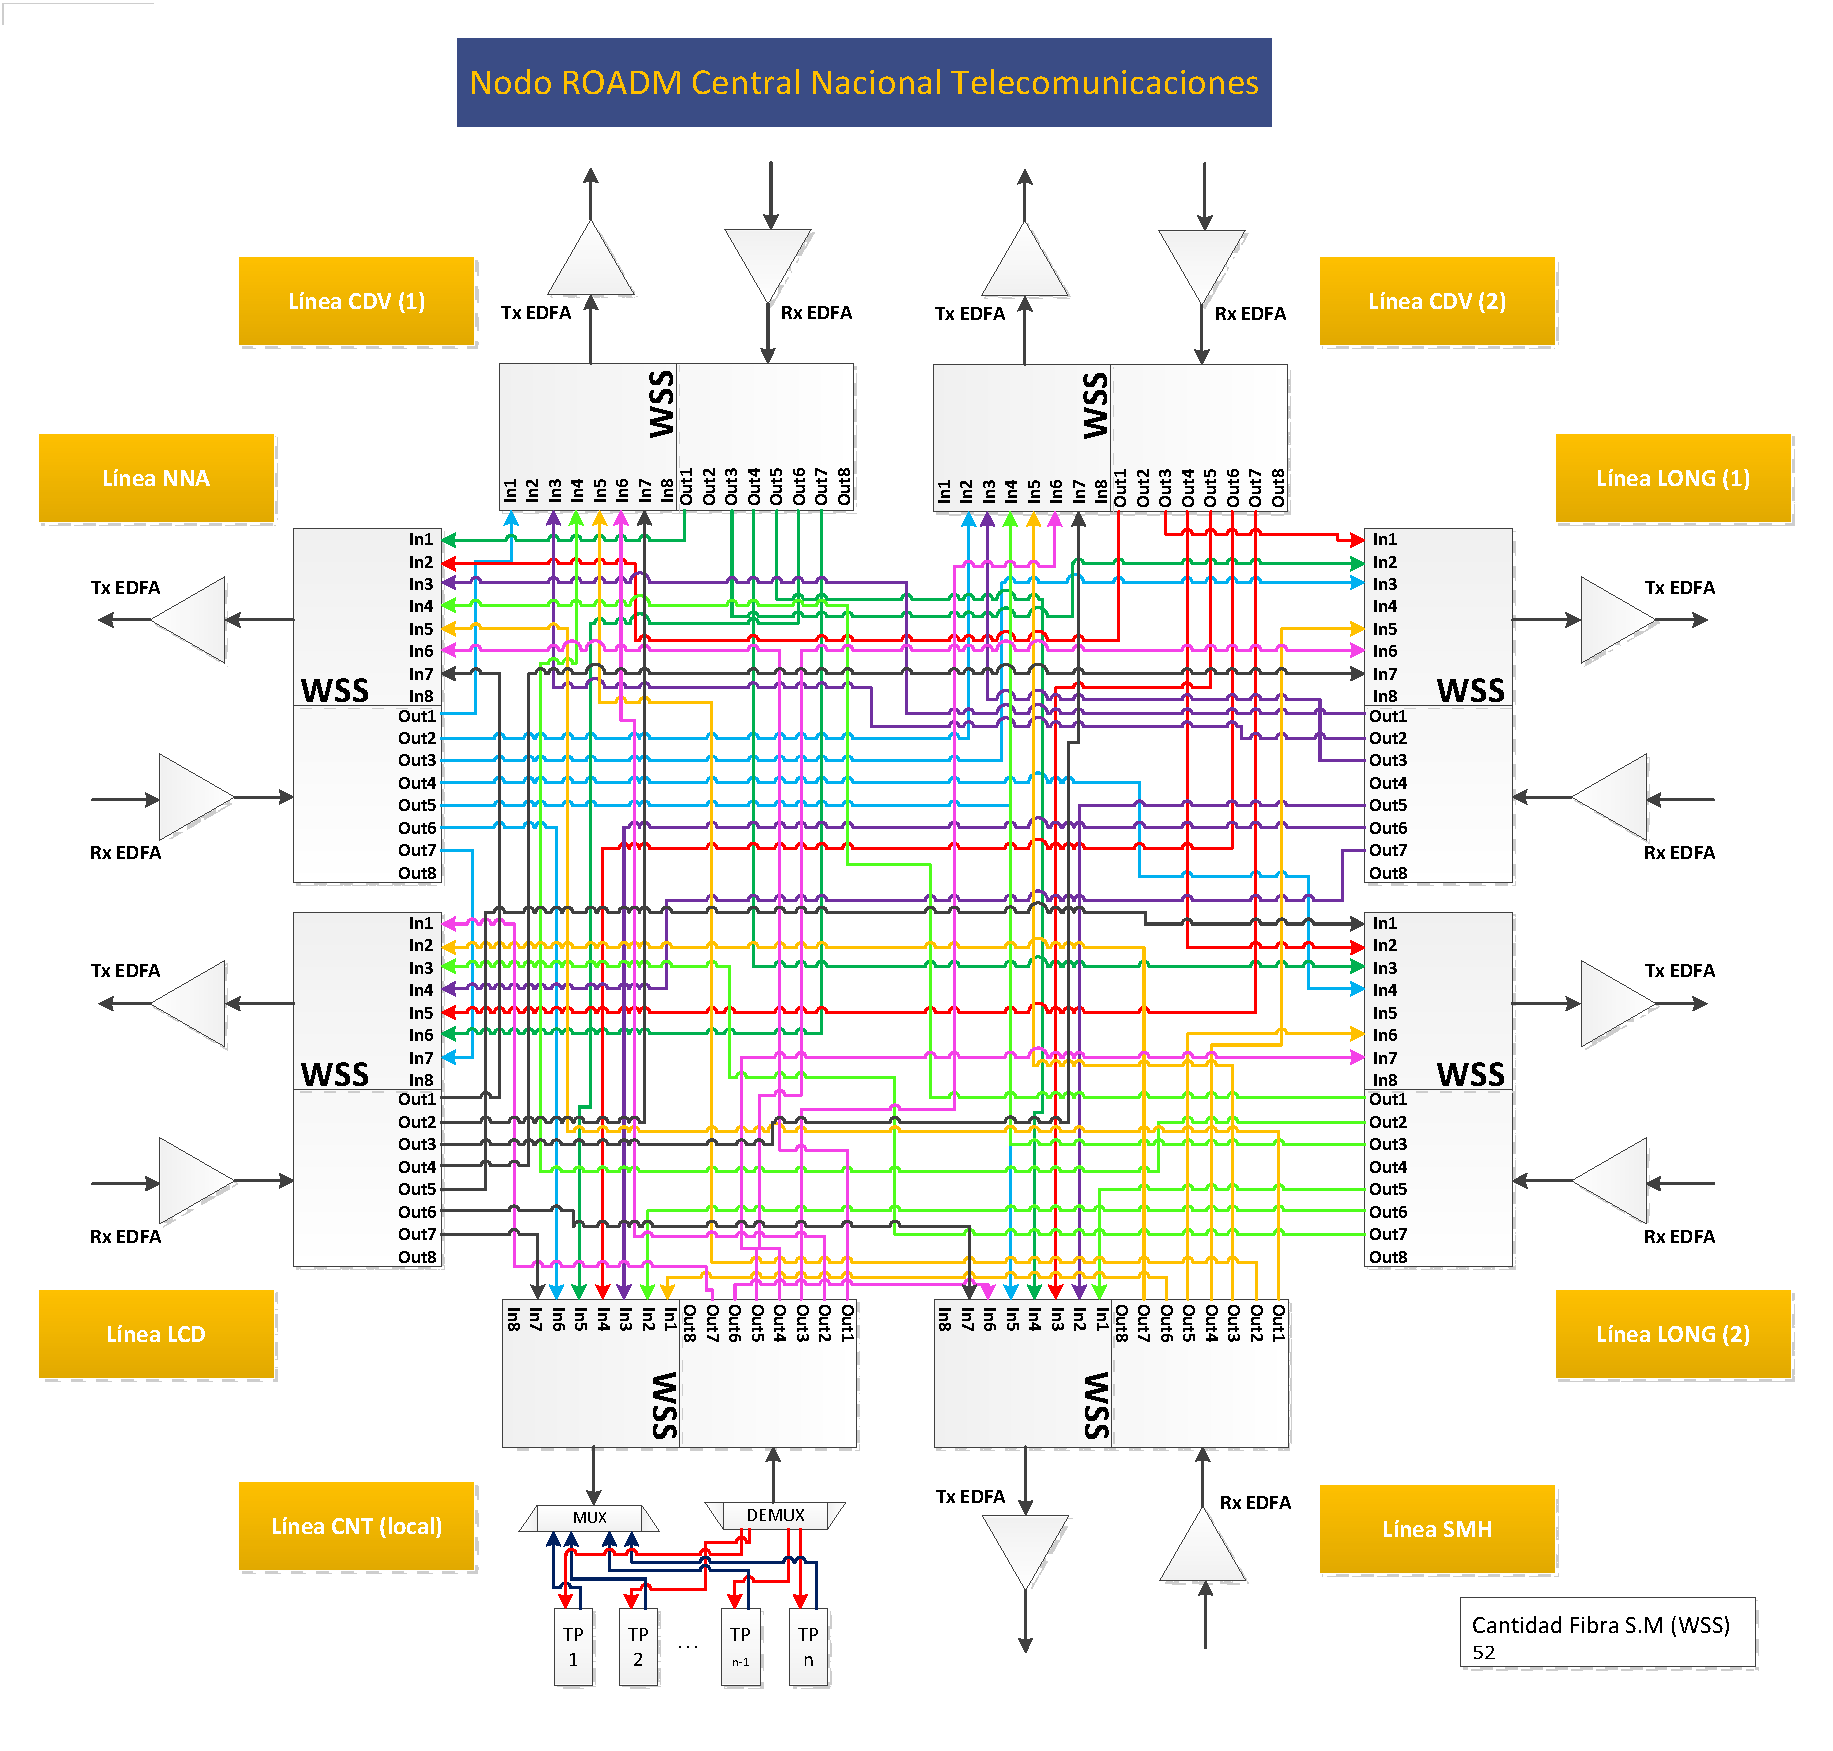
\includegraphics[width=17cm]{Imagenes/CNT.pdf}
  \caption{Diagrama de conexión de equipos para infrastructura ROADM en ``Central nacional de telecomunicaciones''}
  \label{fig:drcnt}
\end{figure}

\subsubsection{Conexión ROADM ``Las Condes''}
\label{sec:drlcd}

\begin{figure}[H]
  \centering
  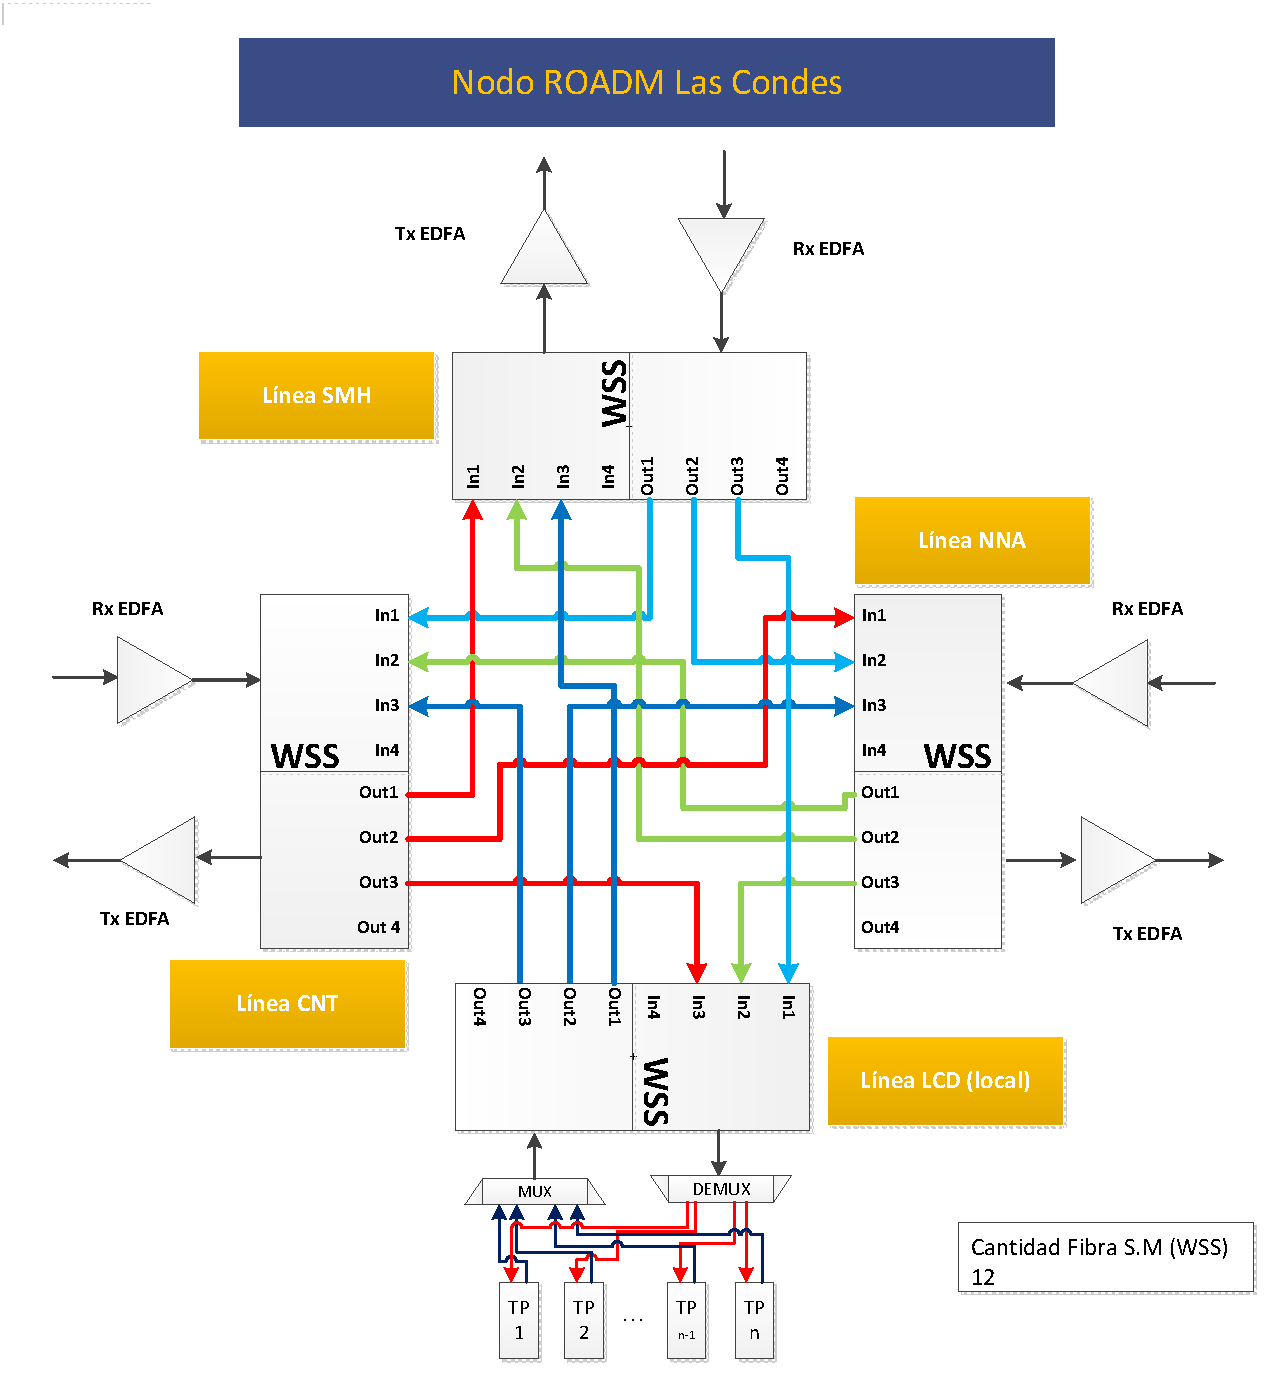
\includegraphics[width=17cm]{Imagenes/LCD.pdf}
  \caption{Diagrama de conexión de equipos para infrastructura ROADM en ``Las Condes''}
  \label{fig:drlcd}
\end{figure}

\subsubsection{Conexión ROADM ``Longovilo''}
\label{sec:drlong}

\begin{figure}[H]
  \centering
  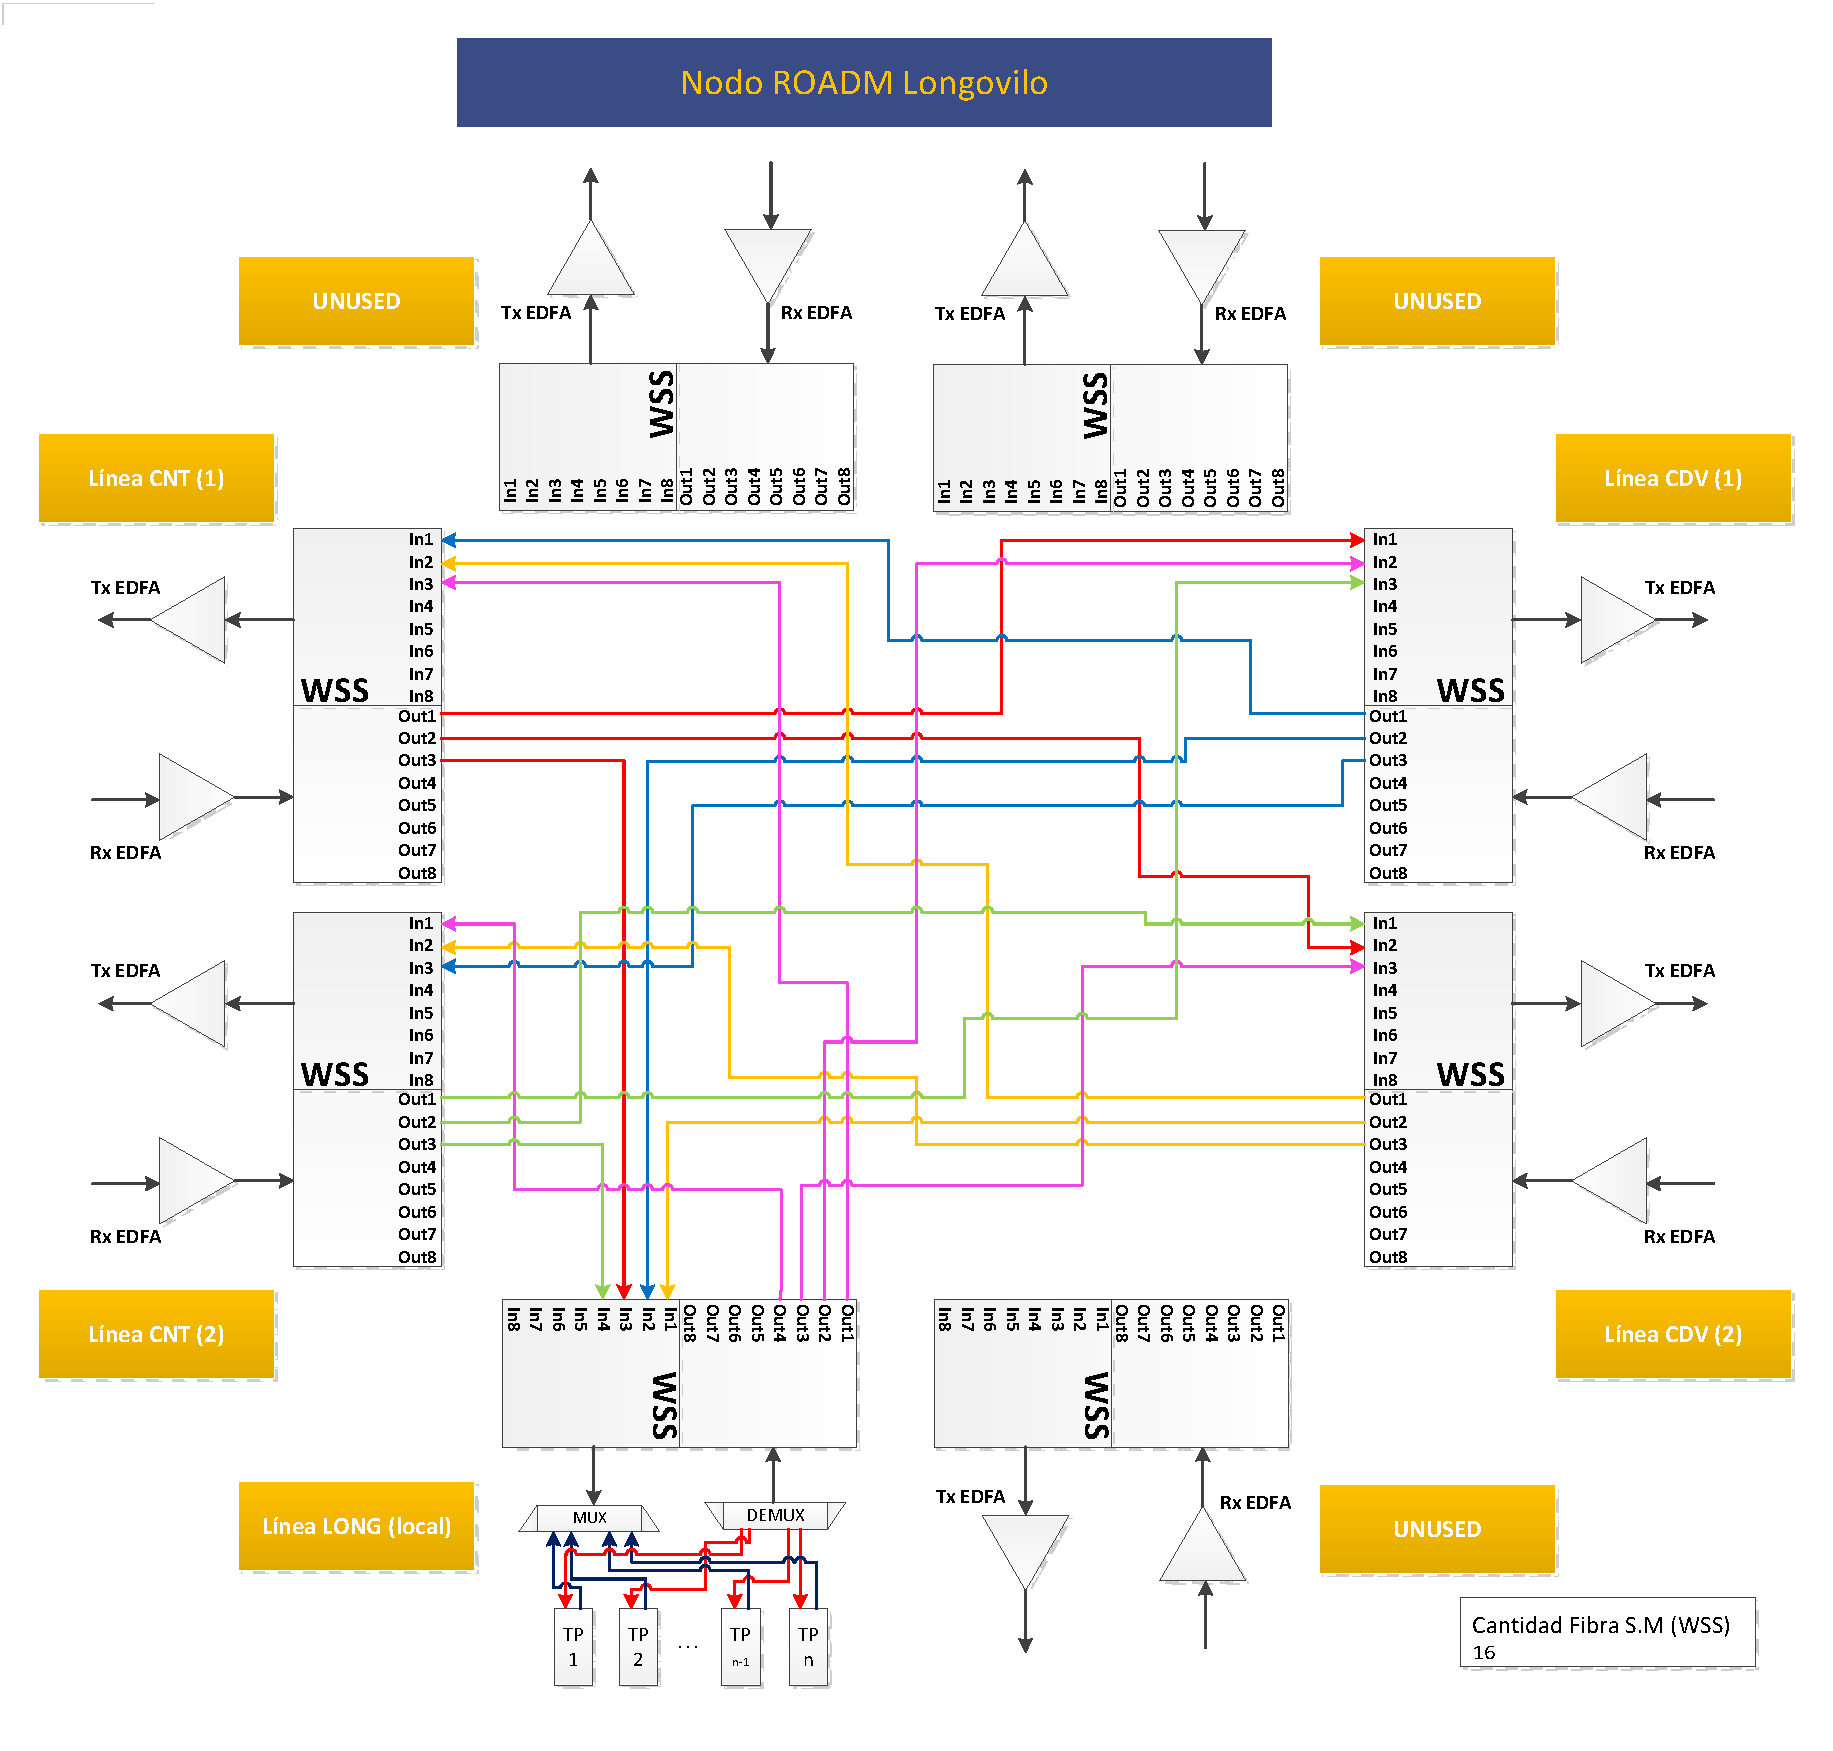
\includegraphics[width=17cm]{Imagenes/LONG.pdf}
  \caption{Diagrama de conexión de equipos para infrastructura ROADM en ``Longovilo''}
  \label{fig:drlong}
\end{figure}

\subsubsection{Conexión ROADM ``Ñuñoa''}
\label{sec:drnna}

\begin{figure}[H]
  \centering
  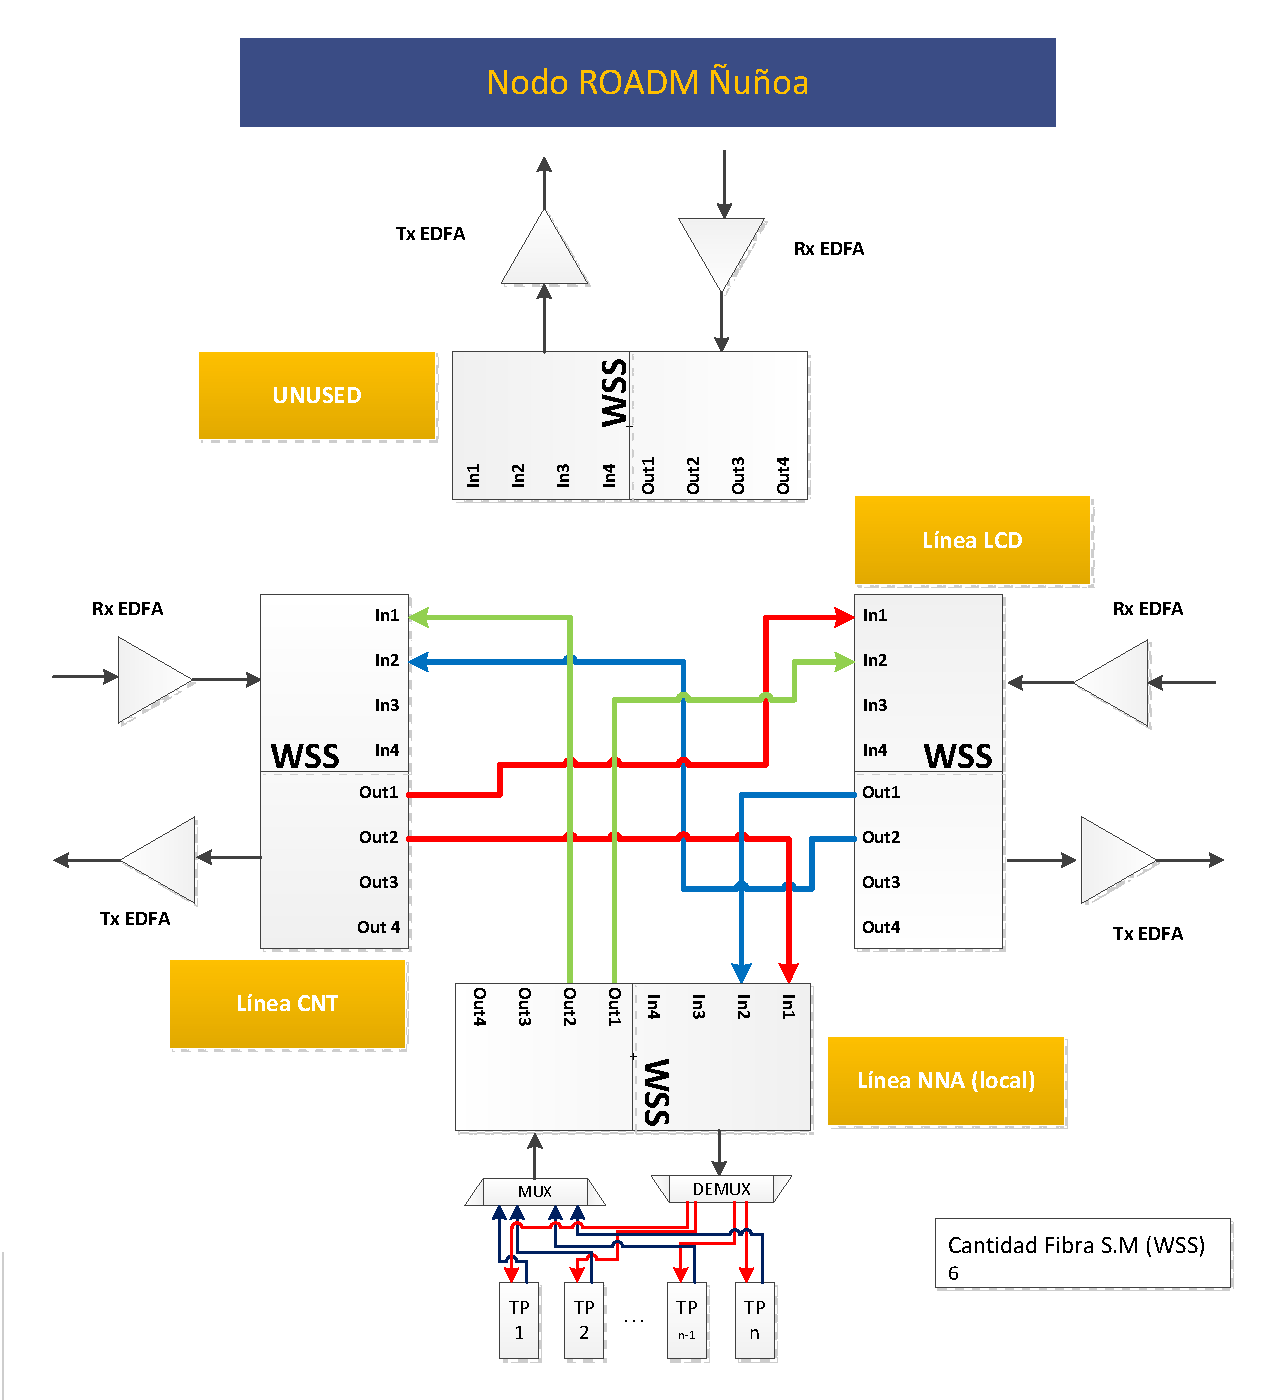
\includegraphics[width=17cm]{Imagenes/NNA.pdf}
  \caption{Diagrama de conexión de equipos para infrastructura ROADM en ``Ñuñoa''}
  \label{fig:drnna}
\end{figure}

\subsubsection{Conexión ROADM ``Santa Marta de Huechuraba''}
\label{sec:drsmh}

\begin{figure}[H]
  \centering
  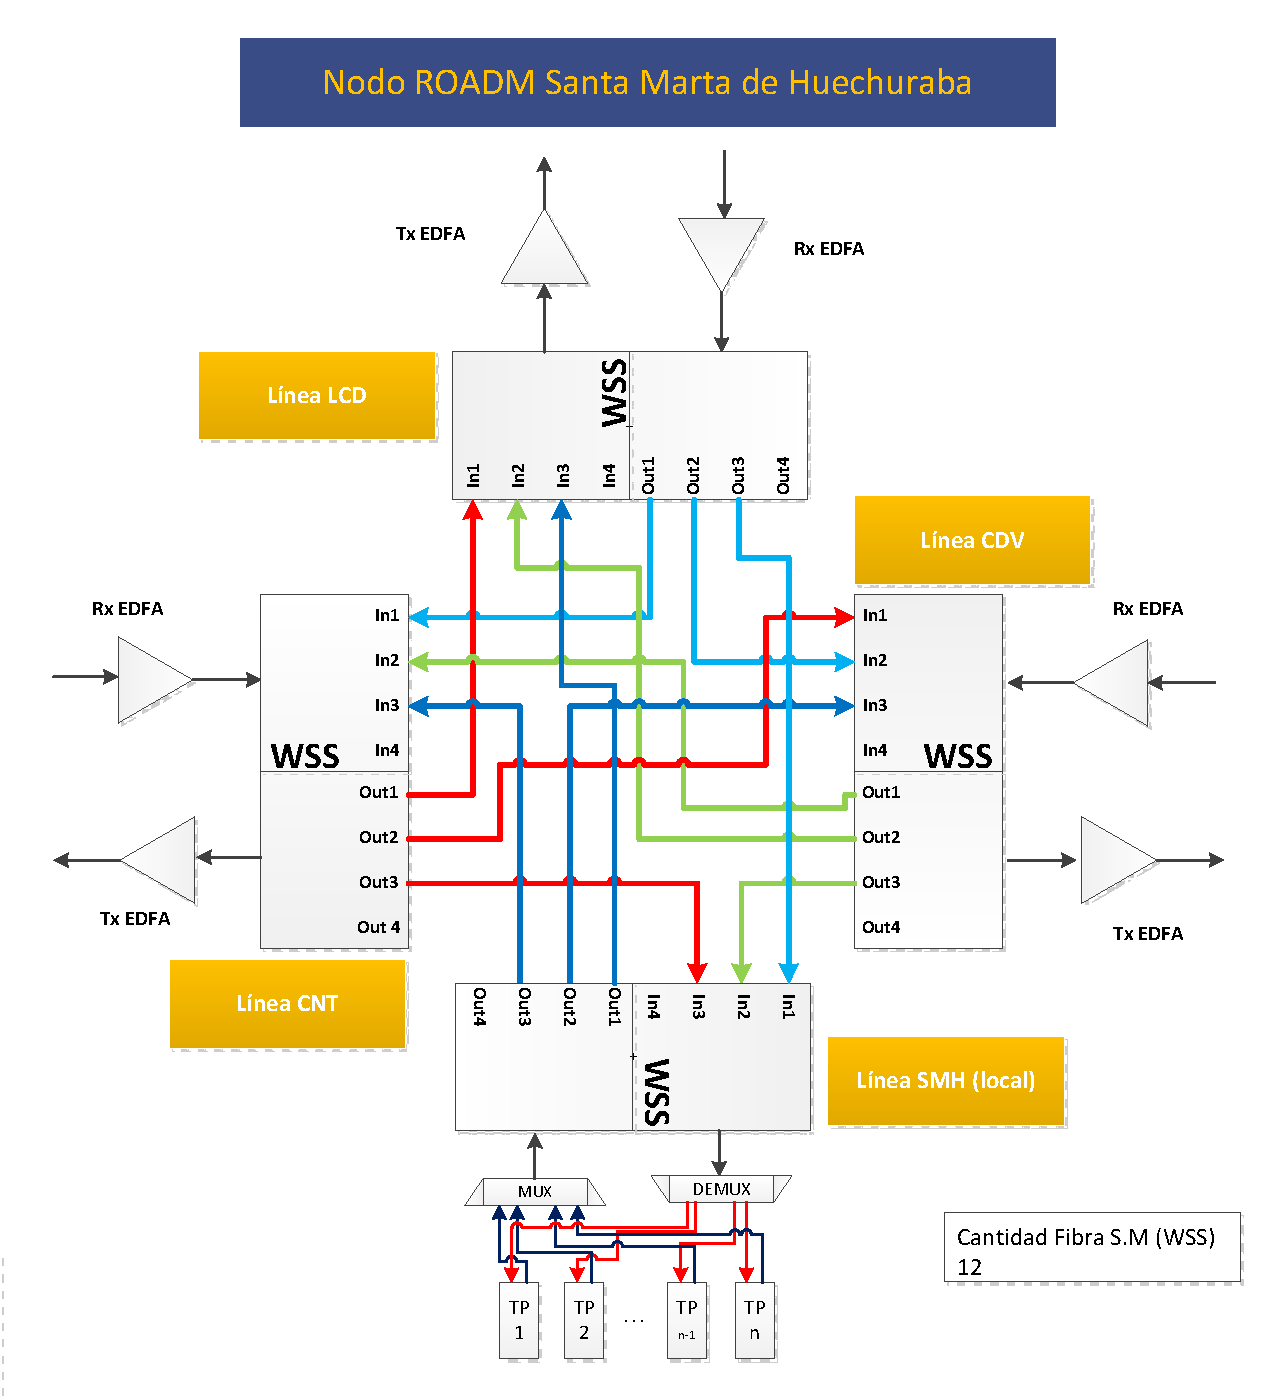
\includegraphics[width=17cm]{Imagenes/SMH.pdf}
  \caption{Diagrama de conexión de equipos para infrastructura ROADM en ``Santa Marta de Huechuraba''}
  \label{fig:drsmh}
\end{figure}

\subsection{Montaje de racks}
\label{sec:racks}

Los racks utilizados en cada \emph{DC} se instalan de la misma manera,
tal y como se muestra en el diagrama \ref{fig:racks}.

\begin{figure}[H]
  \centering
  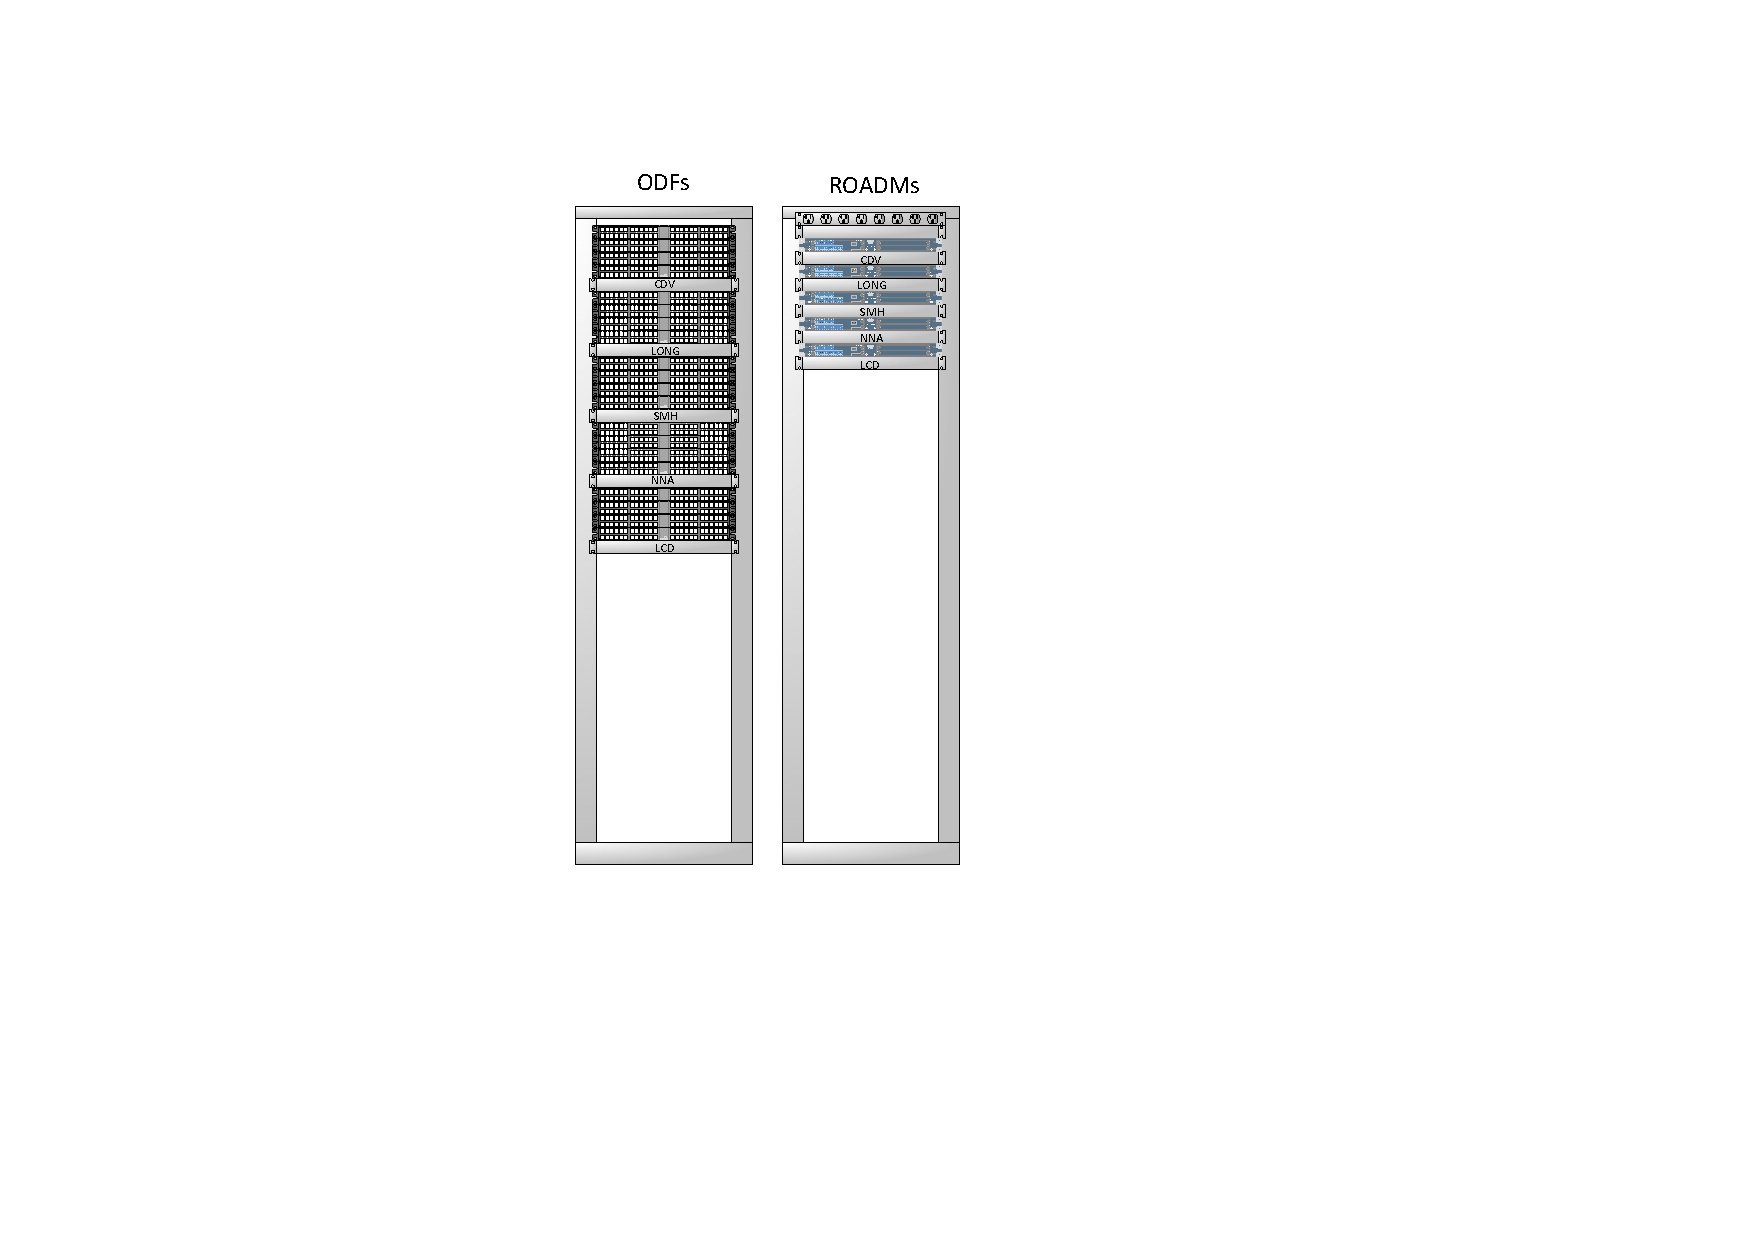
\includegraphics[width=12cm]{Imagenes/racks3.pdf}
  \caption{Montaje de racks en los data centers}
  \label{fig:racks}
\end{figure}

Cada \emph{DC} deberá contar con un rack para albergar y proteger los
ODF (puntos de red de la fibra óptica) y uno para almacenar los
equipos \emph{ROADM}.

El rack de \emph{ROADM}, a su vez, debe seguir las conexiones
mostradas en la sección \ref{sec:diagramasroadm}.

\subsection{Anexo: cálculo OSNR}
\label{sec:osnr}

El \emph{OSNR} (\emph{optical signal to noise ratio}) es la intensidad
de la señal sobre la del ruido en redes ópticas. Se genera en los
\emph{EDFA} (\emph{erbium doped fiber amplifier}), es decir, en los
amplificadores ópticos que no regeneran la señal sino que la
``escalan'' en todas las frecuencias, incluyendo al ruido.

Se puede calcular usando la fórmula: $$n = fgh \nu \Delta \nu$$ donde
$n$ es el nivel de \emph{OSNR}, $f$ es la cifra de ruido del
amplificador, $g$ es la ganancia del mismo, $h$ es la constante de
Planck, $\nu$ es la longitud de onda central de la banda utilizada (en
este caso, la banda C opera sobre los 1550 nm) y $\Delta \nu$ es el
ancho de banda de los canales (en la banda C, el ancho está
aproximadamente por los 0.1 nm). Los tres últimos términos para la
banda C son constantes y se cumple que $$h\nu \Delta \nu \approx -58
dBm$$

Los parámetros $f$ y $g$ son entregados por el fabricante de los
equipos de amplificación y sus unidades son miliWatts.

En el caso de este diseño, los amplificadores existentes en una línea
son dos: el booster y el preamplificador. Por ello, el nivel de ruido
aumenta como la suma de ambos niveles de ruido.

En esta caso los cálculos son los siguientes:
\begin{enumerate}
\item Se identifica la intensidad de la señal útil a la salida del
  preamplificador, es decir, a la entrada del nodo receptor de la
  señal. La señal se calcula como el producto de las ganancias de los
  \emph{EDFA} en la línea dividido por la atenuación total del
  enlace. La atenuación está dada por la distancia y la característica
  de la fibra. Las unidad de este valor es en miliWatts.

  $$p_2=\frac{g_Bg_{PA}}{l}$$

  En este caso, $g_B$ y $g_{PA}$ son iguales a la ganancia del
  amplificador \emph{EDFA} (20 dB = 100 en proporción).
\item Se calcula el ruido a partir de la relación $$n=FGh \nu \Delta
  \nu$$, donde $F$ es el nivel de ruido del amplificador (fijado en 5
  dB), $G$ es la ganancia (fijada en 20 dB) y $h \nu \Delta \nu$ es
  igual $-58dB$.
\item Se hace esto para cada enlace.
\end{enumerate}

Los cálculos de la tabla \ref{tab:osnr1} muestran los resultados de
intensidad de la potencia de la señal al final de cada enlace para
la red propuesta.

\begin{table}[H]
  \centering
  \begin{tabular}{| l | c | c | c | c | c | c |}
    \hline{}
    Enlace & Dist. (Km.) & Atenuac. (dB) \footnote{La atenuación se calculó considerandola lineal como 0.24 dB/Km. de fibra.} & Atenuac. (prop) & $P_out$ (prop) & Ruido (prop) & OSNR (dB) \\
    \hline{}
    CDV-SMH & 30 & 7,2 & 5,25 & 1905,46 & 0,0101 & 52,78 \\
    CDV-LONG & 110 & 26,4 & 436,52 & 22,91 & 0,0006 & 45,70 \\
    CDV-CNT & 45 & 10,8 & 12,02 & 831,76 & 0,0047 & 52,51 \\
    SMH-CNT & 20 & 4,8 & 3,02 & 3311,31 & 0,0171 & 52,87 \\
    SMH-LCD & 25 & 6 & 3,98 & 2511,89 & 0,0131 & 52,83 \\
    CNT-LCD & 12 & 2,88 & 1,94 & 5152,29 & 0,0263 & 52,92 \\
    CNT-NNA & 10 & 2,4 & 1,74 & 5754,40 & 0,0293 & 52,93 \\
    NNA-LCD & 15 & 3,6 & 2,29 & 4365,16 & 0,0224 & 52,90 \\
    LONG-CNT & 132 & 31,68 & 1472,31 & 6,79 & 0,0005 & 41,03 \\
    \hline
  \end{tabular}
  \caption{Tabla de valores de intensidad de la señal útil al final del enlace amplificado.}
  \label{tab:osnr1}
\end{table}

El valor de \emph{OSNR} obtenido es satisfactorio para un diseño como
el propuesto, ya que el umbral supera los $18dB$ mínimos de un sistema
que utiliza tranpondedores no coherentes de 10 Gb, como es este el
caso.
